\section{GUI}
% Möglichst schlechtes Beispiel finden...
\frame{
	\frametitle{GUI}
	\vspace{-2mm}
	\begin{center}
		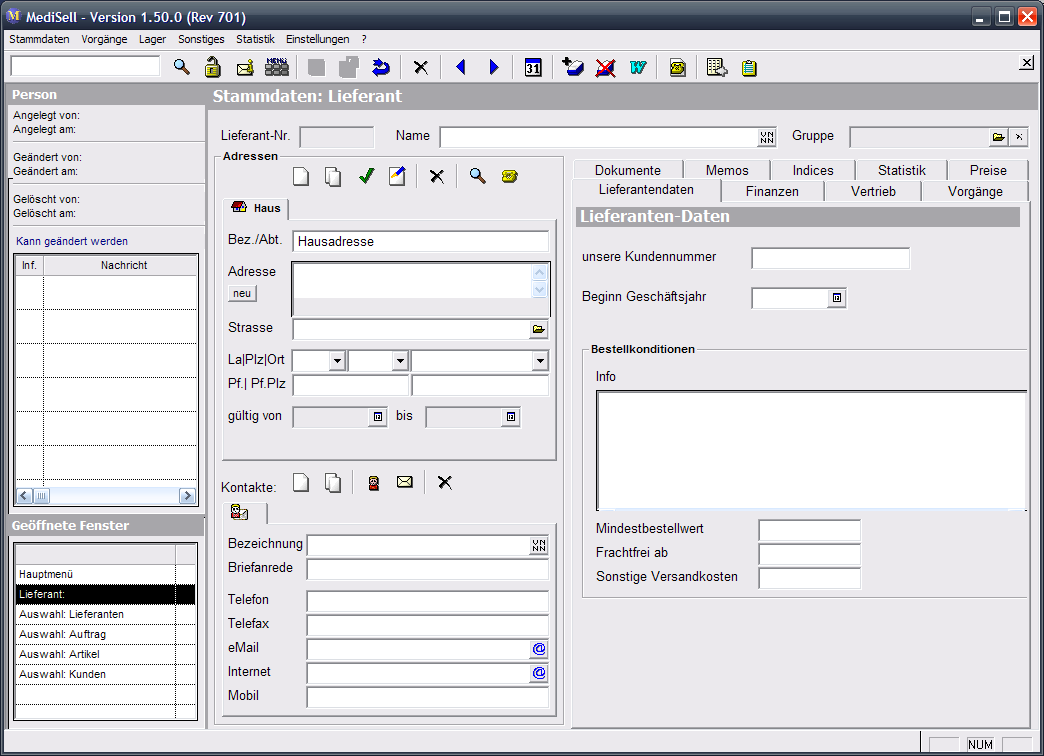
\includegraphics[width=.9\textwidth]{pictures/bad_gui_2.png}
	\end{center}
}
\frame{
	\frametitle{GUI}
	\vspace{-2mm}
	\begin{center}
		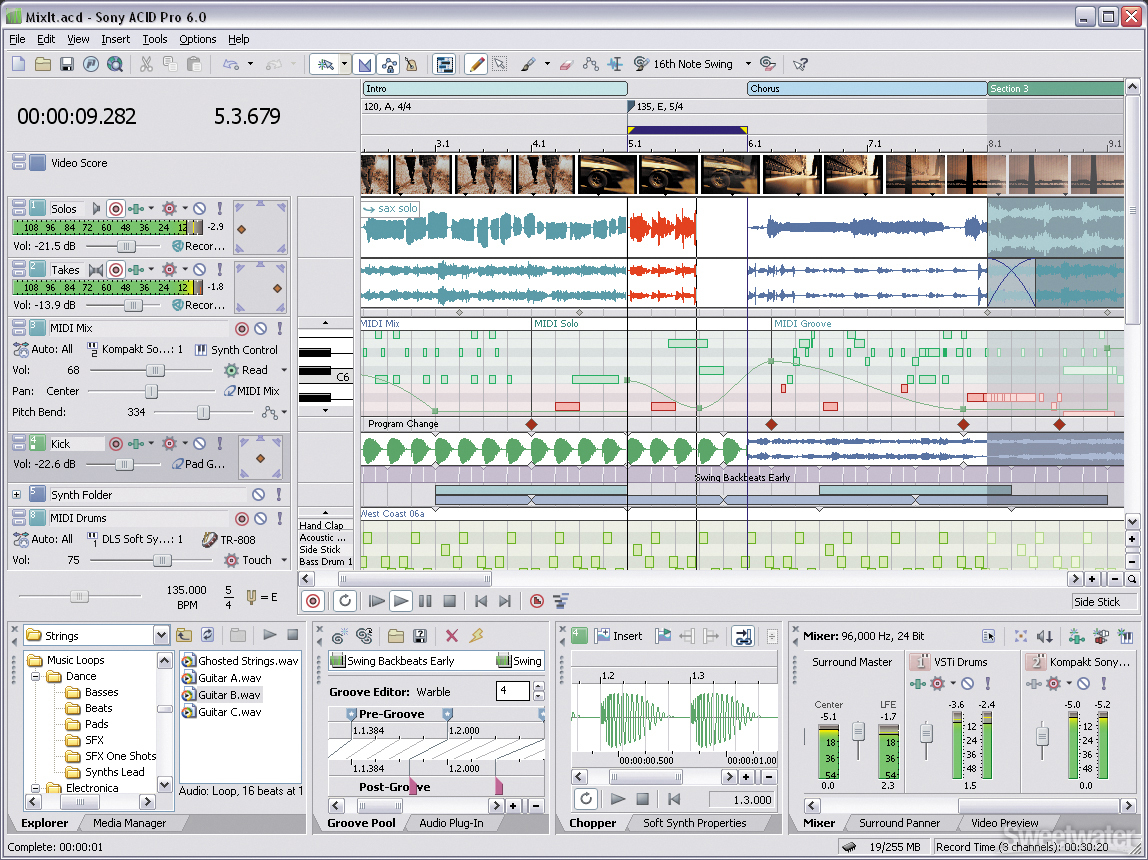
\includegraphics[width=.9\textwidth]{pictures/bad_gui_1.jpg}
	\end{center}
}
\frame{
	\frametitle{GUI}
	\vspace{-2mm}
	\begin{center}
		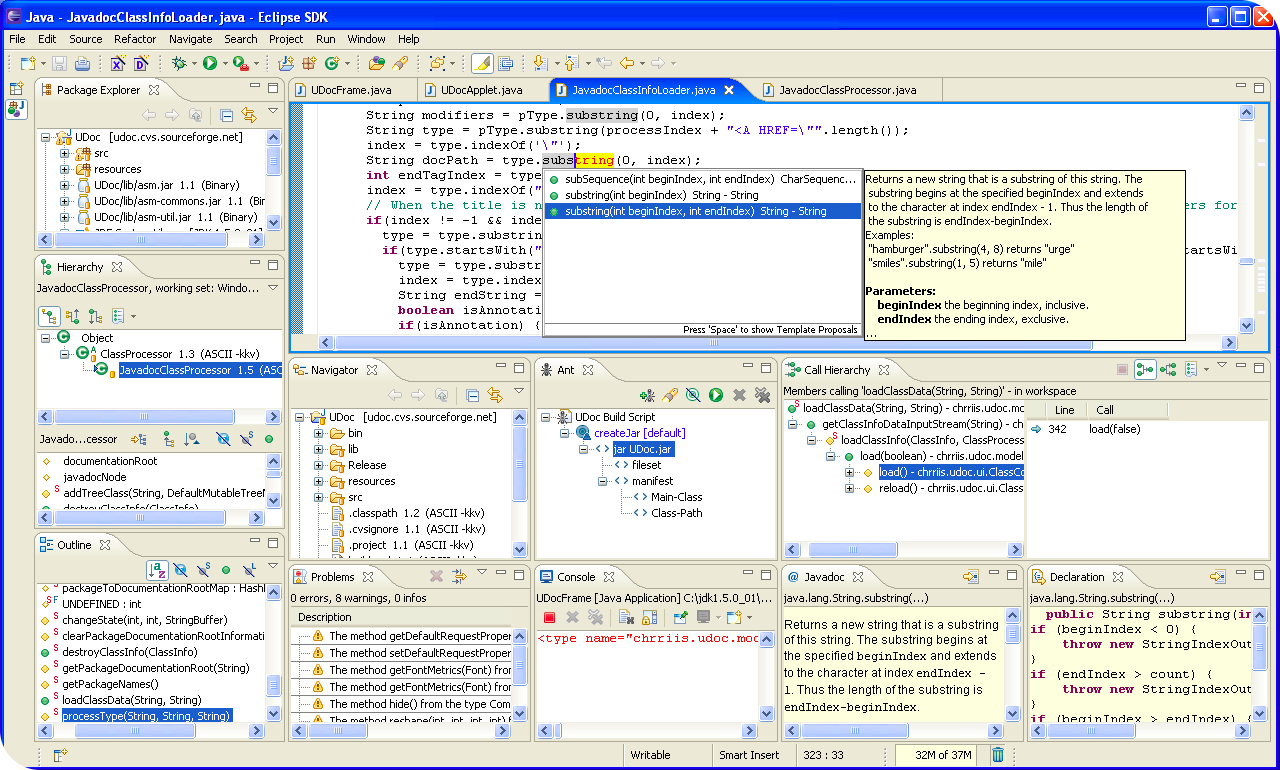
\includegraphics[width=.9\textwidth]{pictures/bad_gui_3.png}
	\end{center}
}
\frame{
	\frametitle{GUI}
	\vspace{-2mm}
	\begin{center}
		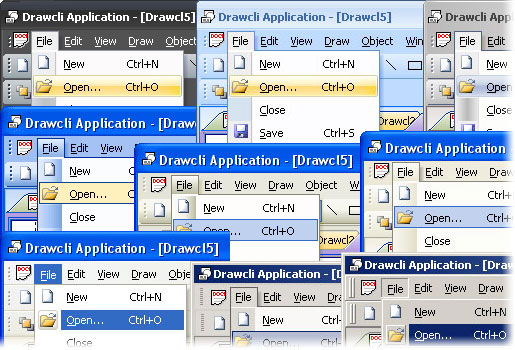
\includegraphics[width=.9\textwidth]{pictures/klickibunti.jpeg}
	\end{center}
}
\frame{
	\frametitle{Besonderheiten bei Smartphones/Tablets}
	\vspace{5mm}
	\begin{itemize}
		\item kleiner Bildschirm \pause
		\vspace{2mm}
		\item Touch-Bedienung \pause
		\vspace{2mm}
		\item verschiedene Größen, Auflösungen und Formate \newline \pause 
		\quad \( \implies \) Größenangaben in px oder cm ungeeignet \pause
		\vspace{2mm}
		\item Drehen des Bildschirms \pause
		\vspace{2mm}
		\item Anwendungskontext (draußen, im Gehen, etc.)
		\vspace{2mm}
		\item \dots
	\end{itemize}
	\vspace{2mm}
	\large{\( \implies \) abstrakte Beschreibung der GUI in XML}
	% ähnlich wie JavaFX, C#, etc.
}

\begin{frame}[fragile]
	\frametitle{XML}
	\vspace{-2mm}
	\begin{lstlisting}[language=XML]
		<Button
		    android:id="@+id/buttonRefresh"
		    android:layout_width="match_parent"
		    android:layout_height="60dp"
		    android:textSize="20sp"
		    android:text="Refresh" />
     \end{lstlisting}
     \pause
     \vspace{-9mm}
     \begin{center}
     	
\includegraphics[width=6cm]{pictures/buttonRefresh.png}
     \end{center}
     \pause
     \vspace{-5mm}
     \begin{itemize}
     	\item \verb|60dp| \textrightarrow \ density-independent pixels \newline
     	\quad \( \implies \) 1 Pixel auf 160 dpi Screen \pause
     	\vspace{2mm}
     	\item \verb|20sp| \textrightarrow \ scale-independent pixels \newline
     	\quad \( \implies \) persönliche Skalierung des Users
     \end{itemize}
\end{frame}

\begin{frame}[fragile]
	\frametitle{XML}
	\vspace{-2mm}
	\begin{lstlisting}[language=XML]
		<TextView
		    android:id="@+id/textViewTemperature"
		    android:layout_width="wrap_content"
		    android:layout_height="wrap_content"
		    android:textSize="50sp"
		    android:text="23 C" />
     \end{lstlisting}
     \pause
     \vspace{-9mm}
     \begin{center}
     	
\includegraphics[width=2cm]{pictures/textViewTemperature.png}
     \end{center}
     \pause
     \vspace{-5mm}
     \begin{itemize}
     	\item \verb|wrap_content| \textrightarrow \ Breite/Höhe passt auf Inhalt \pause
     	\vspace{2mm}
     	\item \verb|match_parent| \textrightarrow \ Breite/Höhe passt auf Rahmen
     \end{itemize}
\end{frame}

\begin{frame}[fragile]
	\frametitle{Layouts}
	\vspace{-2mm}
	\begin{lstlisting}[language=XML]
		<LinearLayout
		    android:layout_width="match_parent"
		    android:layout_height="match_parent"
		    android:orientation="vertical" >

		    <TextView
		        ... />
		    <TextView
		        ... />

		</LinearLayout>
    \end{lstlisting}
\end{frame}

\begin{frame}[fragile]
	\frametitle{Layouts}
	\vspace{-2mm}
	\begin{lstlisting}[language=XML]
		<RelativeLayout
		    android:layout_width="match_parent"
		    android:layout_height="match_parent" >

		    <TextView
		        android:id="@+id/textView1"
		        android:layout_alignParentTop="true"
		        android:layout_centerHorizontal="true"
		        ... />
		    <TextView
		        android:id="@+id/textView2"
		        android:layout_below="@id/textView1"
		        android:layout_centerHorizontal="true"
		        ... />
		</RelativeLayout>
    \end{lstlisting}
\end{frame}

\begin{frame}[fragile]
	\frametitle{Layouts}
	\vspace{-2mm}
	\begin{lstlisting}[language=XML]
		<TableLayout
		    android:layout_width="match_parent"
		    android:layout_height="match_parent" >

		    <TableRow>
		        <TextView
		        ... />
		        <TextView
		        ... />
		    </TableRow>

		    <TableRow> ... </TableRow>

		</TableLayout>
    \end{lstlisting}
\end{frame}

\begin{frame}[fragile]
	\frametitle{Zugriff in Java}
	\begin{lstlisting}[language=Java]
		protected void onCreate(Bundle bundle) {
		    super.onCreate(bundle);

		    // define the layout for this activity
		    setContentView(R.layout.activity_main);
		    
		    // get a reference to the view elements
		    buttonRefresh = (Button)
		        findViewById(R.id.buttonRefresh);
		    textViewTemperature = (TextView)
		        findViewById(R.id.textViewTemperature);
		}
    \end{lstlisting}
\end{frame}

\begin{frame}[fragile]
	\frametitle{Zugriff in Java}
	\begin{lstlisting}[language=Java]
		// manipulate the UI
		textViewTemperature.setText("30")

		//react to UI actions
		buttonRefresh.setOnClickListener(
		    new View.OnClickListener() {
		        public void onClick(View v) {
		            //refresh
		        }
		    });
    \end{lstlisting}
\end{frame}



	% TODO

	% Übertriebenes Klickibunti-Bild
	% GUI wird in XML definiert
	% In Java holt man sich Referenzen darauf und kann es dann manipulieren
	% Layouts:
		% LinearLayout
		% TableLayout
		% RelativeLayout
